\documentclass[letterpaper,12pt]{article}
\usepackage{amsmath}  % improve math presentation
\usepackage{graphicx} % takes care of graphic including machinery
\graphicspath{ {../images/} }
\usepackage{float}
\usepackage[margin=0.8in,letterpaper]{geometry} % decreases margins
\usepackage{longtable}


\begin{document}

\title{Neural Network Model of the Eppler 231 Airfoil Based on Wind Tunnel Data}
\author{Jean de Becdelievre}
\date{\today}
\maketitle

% \section{Nomenclature}

% {\renewcommand\arraystretch{1.0}
% \noindent\begin{longtable}{@{}l @{\quad : \quad} l@{}}
% $L, C_L$ & lift, lift coefficient \\
% $D, C_D$ & drag, drag coefficient \\
% $m, C_m$ & pitching moment, pitching moment coefficient \\
% \end{longtable}}

\begin{figure}[H]
    \centering
    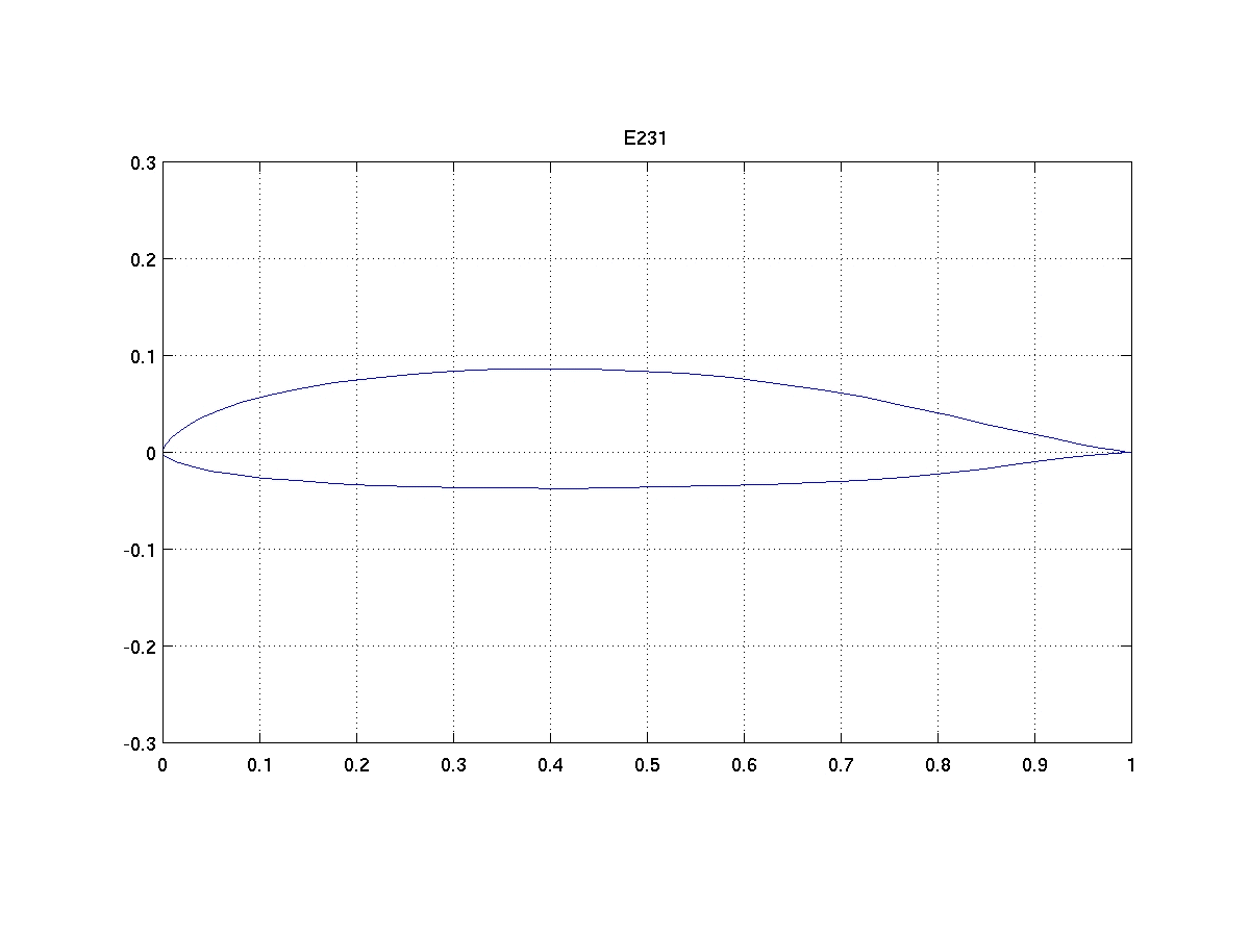
\includegraphics[width=0.6\textwidth]{e231}
    \label{fig:outline}%
\end{figure}

\section{Data}

There are 2 batches of data:
\begin{enumerate}
    \item $C_L$ and $C_m$ only
    \begin{itemize}
        \item 245 measurements
        \item $Re$ range: $[61100, 402800]$
        \item Angle of attack range: $[-6.2, 19.32]$ degrees
    \end{itemize}

    \item $C_L$ and $C_D$ only
    \begin{itemize}
        \item 81 measurements
        \item $Re$ range: $[60800, 400400]$
        \item Angle of attack range: $[-4.57, 11.86]$ degrees
    \end{itemize}

Below are plots of both batches of data.
The second batch is the more interesting one, because it allows to build a polar curve.

\begin{figure}[H]
    \centering
    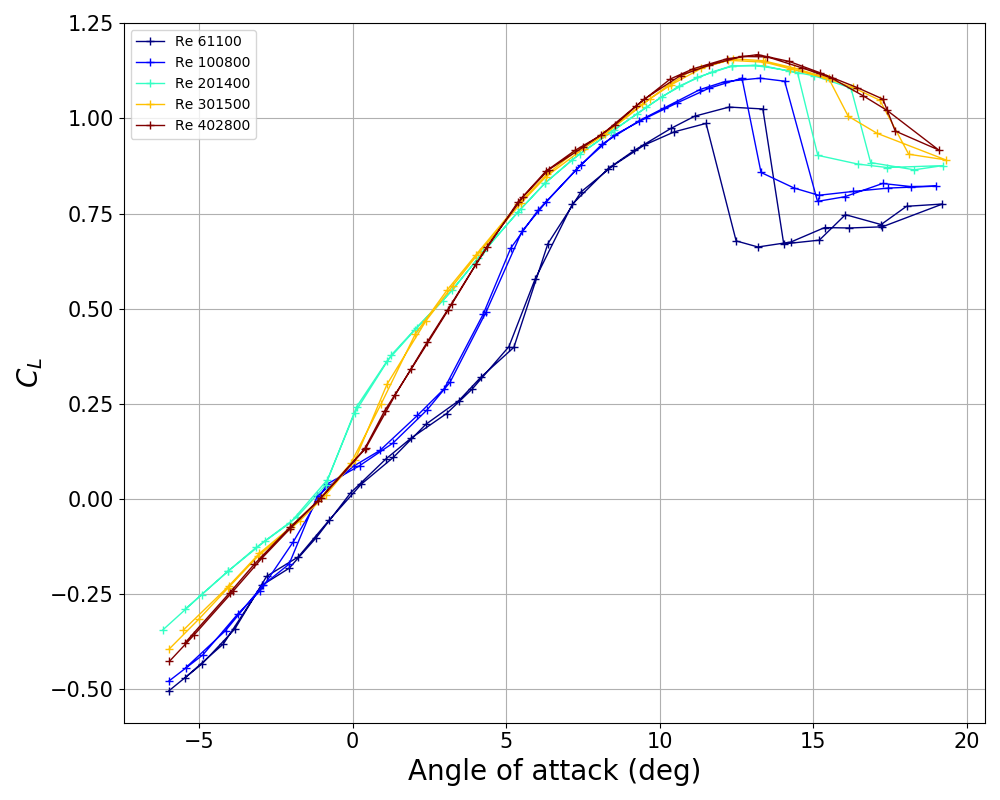
\includegraphics[width=0.7\textwidth]{dataCm_Cl}
    \caption{Batch 1: $C_l$ versus angle of attack}%
    \label{fig:cmcl}%
\end{figure}

\begin{figure}[H]
    \centering
    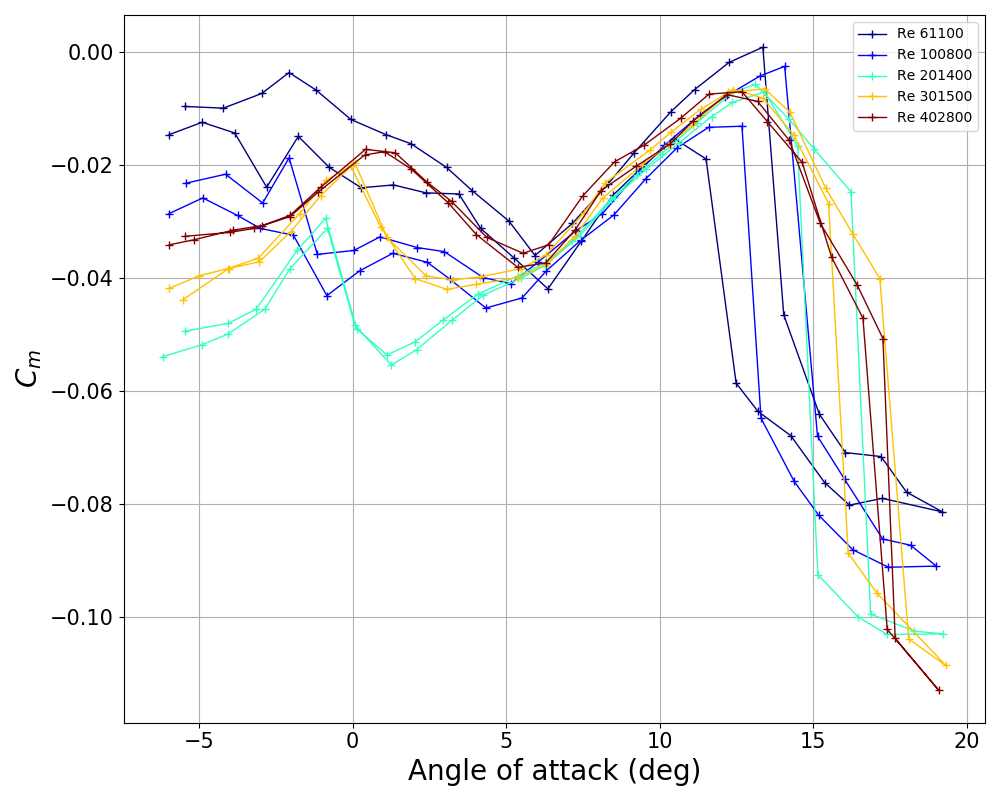
\includegraphics[width=0.7\textwidth]{dataCm}
    \caption{Batch 1: $C_m$ versus angle of attack}%
    \label{fig:cm}%
\end{figure}

\begin{figure}[H]
    \centering
    \includegraphics[width=0.7\textwidth]{dataCd_Cl}
    \caption{Batch 2: $C_L$ versus angle of attack}%
    \label{fig:cdcl}%
\end{figure}

\begin{figure}[H]
    \centering
    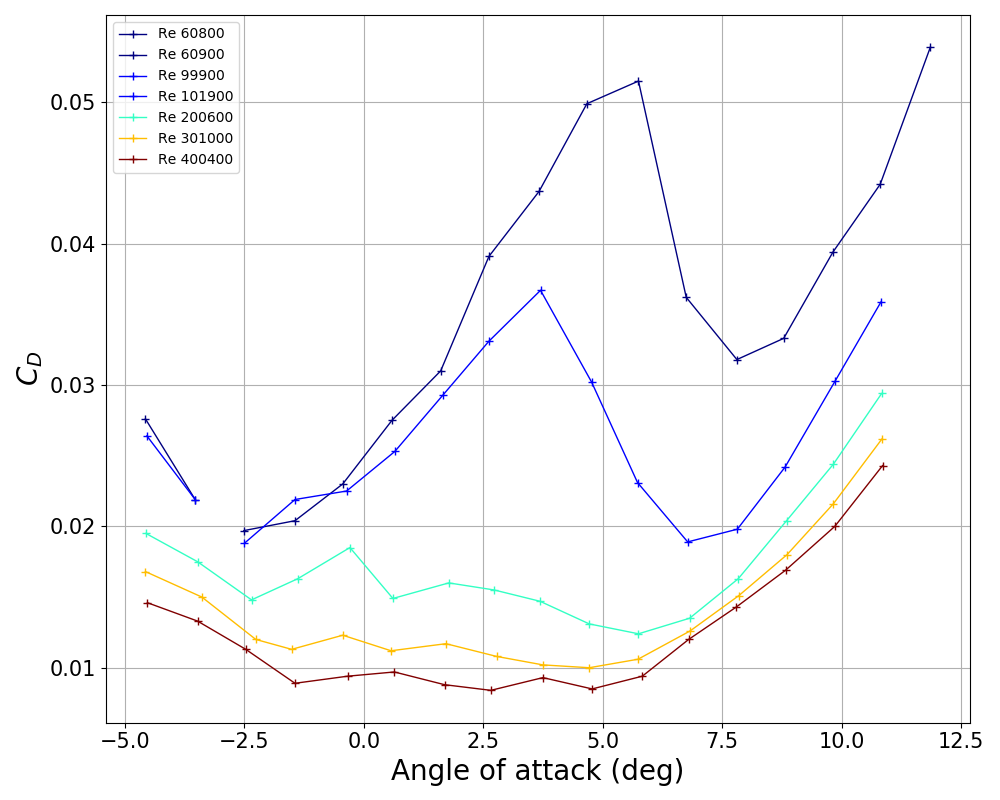
\includegraphics[width=0.7\textwidth]{dataCd}
    \caption{Batch 2: $C_D$ versus angle of attack}%
    \label{fig:cd}%
\end{figure}

\section{Polar fit}

To create an airfoil polar curve, only the second dataset can be used, which only leaves 81 data points. 
The data was fitted using a 1 hidden layer neural network of 8 units, 
with gradient descent and a learning rate of 0.002 for 10000 steps.
Importantly, the very limited amount of data made testing challenging, and a future work includes a proper cross-validation test loss.
The root mean square error on the train set was $0.004$.
% Plots below show the function's prediction on the training data, as well as some contours:
\vspace{-1cm}

\begin{figure}[H]
    \centering
    \includegraphics[width=0.7\textwidth]{nn_pred}
    \vspace{-1cm}
    \caption{Neural network prediction versus training data}%
    \label{fig:nn_pred}%
\end{figure}

\begin{figure}[H]
    \centering
    \includegraphics[width=0.7\textwidth]{nn}
    \vspace{-0.7cm}
    \caption{Contour plot of the neural network fit}%
    \label{fig:nn}%
\end{figure}

\end{enumerate}

\end{document}
